\documentclass[12pt]{beamer}
\usepackage{../Estilos/BeamerMAF}
\usepackage[absolute, overlay]{textpos}
\usepackage{../Estilos/ColoresLatex}
%Sección para el tema de beamer, con el theme, usercolortheme y sección de footers
\usetheme{Antibes}
\usecolortheme{beaver}
%\useoutertheme{default}
\setbeamercovered{invisible}
% or whatever (possibly just delete it)
\setbeamertemplate{section in toc}[sections numbered]
\setbeamertemplate{subsection in toc}[subsections numbered]
\setbeamertemplate{subsection in toc}{\leavevmode\leftskip=3.2em\rlap{\hskip-2em\inserttocsectionnumber.\inserttocsubsectionnumber}\inserttocsubsection\par}
\setbeamercolor{section in toc}{fg=blue}
\setbeamercolor{subsection in toc}{fg=blue}
%\setbeamercolor{frametitle}{fg=blue}
\setbeamertemplate{caption}[numbered]

\setbeamertemplate{footline}
\beamertemplatenavigationsymbolsempty
\setbeamertemplate{headline}{}


\makeatletter
\setbeamercolor{secºtion in foot}{bg=gray!30, fg=black!90!orange}
\setbeamercolor{subsection in foot}{bg=blue!30!yellow, fg=red}
\setbeamercolor{date in foot}{bg=black, fg=white}
\setbeamertemplate{footline}
{
  \leavevmode%
  \hbox{%
  \begin{beamercolorbox}[wd=.333333\paperwidth,ht=2.25ex,dp=1ex,center]{section in foot}%
    \usebeamerfont{section in foot} \insertsection
  \end{beamercolorbox}%
  \begin{beamercolorbox}[wd=.333333\paperwidth,ht=2.25ex,dp=1ex,center]{subsection in foot}%
    \usebeamerfont{subsection in foot}  \insertsubsection
  \end{beamercolorbox}%
  \begin{beamercolorbox}[wd=.333333\paperwidth,ht=2.25ex,dp=1ex,right]{date in head/foot}%
    \usebeamerfont{date in head/foot} \insertshortdate{} \hspace*{2em}
    \insertframenumber{} / \inserttotalframenumber \hspace*{2ex} 
  \end{beamercolorbox}}%
  \vskip0pt%
}







\setbeamercolor{section in foot}{bg=amethyst, fg=white}
\setbeamercolor{subsection in foot}{bg=almond, fg=black}

\makeatletter
\setbeamertemplate{footline}
{
\leavevmode%
\hbox{%
\begin{beamercolorbox}[wd=.333333\paperwidth,ht=2.25ex,dp=1ex,center]{section in foot}%
  \usebeamerfont{section in foot} \insertsection
\end{beamercolorbox}%
\begin{beamercolorbox}[wd=.333333\paperwidth,ht=2.25ex,dp=1ex,center]{subsection in foot}%
  \usebeamerfont{subsection in foot}  \insertsubsection
\end{beamercolorbox}%
\begin{beamercolorbox}[wd=.333333\paperwidth,ht=2.25ex,dp=1ex,right]{date in head/foot}%
  \usebeamerfont{date in head/foot} \insertshortdate{} \hspace*{1.5em}
  \insertframenumber{} / \inserttotalframenumber \hspace*{2ex} 
\end{beamercolorbox}}%
\vskip0pt%
}
\makeatother
% \usefonttheme{serif}
\setbeamercolor{frametitle}{bg=champagne}
\resetcounteronoverlays{saveenumi}

\AtBeginDocument{\RenewCommandCopy\qty\SI}
\ExplSyntaxOn
\msg_redirect_name:nnn { siunitx } { physics-pkg } { none }
\ExplSyntaxOff

% \date{31 de mayo de 2022}

\title{\large{Tema 6 - Transformadas Integrales}}
\subtitle{Matemáticas Avanzadas de la Física}
\author{M. en C. Gustavo Contreras Mayén}

\begin{document}
\maketitle
\fontsize{14}{14}\selectfont
\spanishdecimal{.}

\section*{Contenido}
\frame[allowframebreaks]{\frametitle{Temas a revisar} \tableofcontents[currentsection, hideallsubsections]}

%Referencia. Debnath - Integral transforms and their applications. Sec. 1.1

% \section{Las Transformadas Integrales}
% \frame[allowframebreaks]{\frametitle{Contenido}\tableofcontents[currentsection, hideothersubsections]}
% \subsection{Introducción}

% \begin{frame}
% \frametitle{Marco histórico}
% Las transformadas integrales se han utilizado con éxito durante casi dos siglos para resolver muchos problemas en matemática aplicada, física matemática y ciencias de la ingeniería.
% \end{frame}
% \begin{frame}
% \frametitle{Marco histórico}
% Históricamente, el origen de las transformaciones integrales, incluidas las transformadas de Laplace y de Fourier, \pause se remonta a la célebre obra de Laplace (1749-1827) sobre la teoría de la probabilidad en la década de 1780 \pause y al tratado monumental de Joseph Fourier (1768-1830) en \emph{La Théorie Analytique de la Chaleur} publicada en 1822.
% \end{frame}
% \begin{frame}
% \frametitle{Marco histórico}
% De hecho, el libro clásico de Laplace \emph{La Théorie Analytique des Probabilities} incluye algunos resultados básicos de la transformada de Laplace, \pause que es una de las transformadas integrales más antiguas y más utilizadas en la literatura matemática. 
% \end{frame}
% \begin{frame}
% \frametitle{Marco histórico}
% Esto se ha utilizado efectivamente para encontrar la solución de ecuaciones diferenciales lineales y ecuaciones integrales.
% \\
% \bigskip
% \pause
% Por otro lado, el tratado de Fourier proporcionó la teoría matemática moderna de la conducción de calor, las series de Fourier y las integrales de Fourier con aplicaciones.
% \end{frame}
% \begin{frame}
% \frametitle{Marco histórico}
% En su tratado, Fourier declaró un resultado notable que se conoce universalmente como el \textocolor{blue}{Teorema Integral de Fourier}.
% \end{frame}
% \begin{frame}
% \frametitle{Marco histórico}
% Proporcionó una serie de ejemplos antes de afirmar que una función arbitraria definida en un intervalo finito puede expandirse en términos de series trigonométricas que ahora se conocen universalmente como la \textocolor{lava}{serie de Fourier}.
% \end{frame}
% \begin{frame}
% \frametitle{Marco histórico}
% En un intento por extender sus nuevas ideas a funciones definidas en un intervalo infinito, \pause Fourier descubrió una transformada integral y su fórmula de inversión que ahora se conocen como la \textocolor{ao}{transformada de Fourier} y la \textocolor{armygreen}{transformada de Fourier inversa}.
% \end{frame}
% \begin{frame}
% \frametitle{Marco histórico}
% Sin embargo, esta célebre idea de Fourier era conocida por Laplace y Cauchy (1789–1857), ya que algunos de sus trabajos anteriores implicaban esta transformada.
% \end{frame}
% \begin{frame}
% \frametitle{Marco histórico}
% Por otro lado, Poisson (1781–1840) también utilizó de manera independiente el método de transformada en su investigación sobre la propagación de ondas de agua.
% \end{frame}
% \begin{frame}
% \frametitle{Marco histórico}
% Sin embargo, fue Leibniz (1646–1716) quien introdujo por primera vez la idea de un método simbólico en el cálculo.
% \\
% \bigskip
% \pause
% Posteriormente, tanto Lagrange (1736–1813) como Laplace hicieron contribuciones considerables a los métodos simbólicos que se conocieron como cálculo operacional.
% \end{frame}
% \begin{frame}
% \frametitle{Marco histórico}
% Aunque tanto la transformada de Laplace como la de Fourier se descubrieron en el siglo XIX, \pause fue el ingeniero eléctrico británico Oliver Heaviside (1850–1925) quien hizo la transformada de Laplace muy popular al usarla para resolver ecuaciones diferenciales ordinarias de circuitos y sistemas eléctricos, y luego desarrollar el cálculo operacional moderno.
% \end{frame}
% \begin{frame}
% \frametitle{Marco histórico}
% Puede ser relevante señalar que la transformada de Laplace es esencialmente un caso especial de la transformada de Fourier para una clase de funciones definidas en el eje real positivo, pero es más simple que la transformada de Fourier por las siguientes razones:
% \end{frame}
% \begin{frame}
% \frametitle{Marco histórico}
% \setbeamercolor{item projected}{bg=asparagus,fg=white}
% \setbeamertemplate{enumerate items}{%
% \usebeamercolor[bg]{item projected}%
% \raisebox{1.5pt}{\colorbox{bg}{\color{fg}\footnotesize\insertenumlabel}}%
% }
% \begin{enumerate}[<+->]
% \item La cuestión de la convergencia de la transformada de Laplace es mucho menos delicada debido al kernel de la exponencial decreciente $\exp (-s \, t)$, donde $\Re{s} > 0$ y $t > 0$.
% \seti
% \end{enumerate}
% \end{frame}
% \begin{frame}
% \frametitle{Marco histórico}
% \setbeamercolor{item projected}{bg=asparagus,fg=white}
% \setbeamertemplate{enumerate items}{%
% \usebeamercolor[bg]{item projected}%
% \raisebox{1.5pt}{\colorbox{bg}{\color{fg}\footnotesize\insertenumlabel}}%
% }
% \begin{enumerate}[<+->]
% \conti
% \item La transformada de Laplace es una función analítica de variable compleja y sus propiedades pueden ser fácilmente estudiadas con el conocimiento de la teoría de la variable compleja.
% \seti
% \end{enumerate}
% \end{frame}
% \begin{frame}
% \frametitle{Marco histórico}
% \setbeamercolor{item projected}{bg=asparagus,fg=white}
% \setbeamertemplate{enumerate items}{%
% \usebeamercolor[bg]{item projected}%
% \raisebox{1.5pt}{\colorbox{bg}{\color{fg}\footnotesize\insertenumlabel}}%
% }
% \begin{enumerate}[<+->]
% \conti
% \item La fórmula integral de Fourier proporcionó las definiciones de la transformada de Laplace y la transformada inversa de Laplace en términos de una integral de contorno complejo que se puede evaluar con la ayuda de la teoría del residuo de Cauchy y la deformación del contorno en el plano complejo.
% \end{enumerate}
% \end{frame}

\section{Conceptos básicos}
\frame[allowframebreaks]{\frametitle{Temas a revisar} \tableofcontents[currentsection, hideothersubsections]}
\subsection{Definición}

\begin{frame}
\frametitle{Definición de la transformada integral}
La transformada integral de una función $f (x)$ definida en el intervalo $a \leq x \leq b$, se escribe como $\mathscr{I} \left\{ f (x) \right\} = F (x)$ y se define por:
\pause
\begin{align}
\mathscr{I} \left\{ f (x) \right\} = F (k) = \scaleint{6ex}_{\bs a}^{b} K (x, k) \, f (x) \dd{x}
\label{eq:ecuacion_01_02_01}
\end{align}
\end{frame}
\begin{frame}
\frametitle{Definición de la transformada integral}
\begin{align*}
\mathscr{I} \left\{ f (x) \right\} = F (k) = \scaleint{6ex}_{\bs a}^{b} K (x, k) \, f (x) \dd{x}
\end{align*}
donde $K (x, k)$ es una función dada de dos variables $x$ y $k$, que se le llama \textbf{\textcolor{blue(pigment)}{kernel}} de la transformada.
\end{frame}
\begin{frame}
\frametitle{La transformada}
El operador $\mathscr{I}$ es llamada \emph{operador de transformada integral} o simplemente \textbf{\textcolor{brickred}{transformada integral}}.
\\
\bigskip
\pause
La función transformada $F (k)$ se refiera a menudo como la \emph{imagen} de la función dada $f (x)$, y $k$ es llamada la \emph{variable transformada}.
\end{frame}
\begin{frame}
\frametitle{Transformada de varias variables}
De manera similar, la transformada integral de una función de varias variables se define por:
\pause
\begin{align}
\mathscr{I} \left\{ f (x) \right\} = F(\mathbf{k}) = \scaleint{6ex}_{\bs S} K (\mathbf{x}, \mathbf{k}) \, f (\mathbf{x}) \dd{x}
\label{eq:ecuacion_01_02_02}
\end{align}
donde $\mathbf{x} = (x_{1}, x_{2}, \ldots, x_{n}), \mathbf{k} = (k_{1}, k_{2}, \ldots, k_{n})$ y $S \in R^{n}$.
\end{frame}

% %Referencia Arfken - Mathematical methods for physicists. Cap. 15 Integral Transforms -djvu
% % \section{Transformadas Integrales.}
% % Frecuentemente en física uno se encuentra con pares de funciones que se encuentran relacionadas por una expresión como la siguiente
% % \begin{equation}
% % g (\alpha) = \scaleint{6ex}_{\bs a}^{b} f (t) \, K(\alpha, t) \, \dd t
% % \label{eq:ecuacion_15_01}
% % \end{equation}
% % La función $g (\alpha)$ es llamada la transformada integral de $f (t)$ por el núcleo (o kernel)  $K (\alpha,t)$.
% \par
% La operación de transformación se puede describir como un mapeo de una función $f (t)$ en el espacio-$t$ a otra función $F (\alpha)$ en el espacio-$\alpha$. Dos ejemplos de esta interpretación en física son las relaciones entre: el tiempo y la frecuencia en electrodinámica clásica y mecánica cuántica, y la relación entre el espacio de configuraciones y el espacio de momentos en mecánica cuántica.
% \par
% Cuando los límites de integración $a$ y $b$ son finitos, decimos que $F (\alpha)$ es es la transformada finita de $f (x)$. 

\subsection{Tipos de Transformadas Integrales}

\begin{frame}
\frametitle{Varias Transformadas Integrales}
Existen varios tipos de transformadas integrales que aparecen frecuentemente en la física matemática, \pause cada una de ellas está asociada a un kernel (núcleo) diferente.
\\
\bigskip
\pause
De entre las diferentes posibilidades podemos mencionar los núcleos siguientes:
\end{frame}
\begin{frame}
\frametitle{Lista de Transformadas Integrales}
\setbeamercolor{item projected}{bg=caribbeangreen,fg=black}
\setbeamertemplate{enumerate items}{%
\usebeamercolor[bg]{item projected}%
\raisebox{1.5pt}{\colorbox{bg}{\color{fg}\footnotesize\insertenumlabel}}%
}
\begin{enumerate}[<+->]
\item \emph{Transformada de Fourier.}
\begin{align}
g (\omega) = \dfrac{1}{\sqrt{2 \, \pi}} \scaleint{6ex}_{\bs -\infty}^{\infty} f (t) \, e^{i \omega t} \, \dd{t}
\label{eq:ecuacion_07_01}
\end{align}
\seti
\end{enumerate}
\end{frame}
\begin{frame}
\frametitle{Lista de Transformadas Integrales}
\setbeamercolor{item projected}{bg=caribbeangreen,fg=black}
\setbeamertemplate{enumerate items}{%
\usebeamercolor[bg]{item projected}%
\raisebox{1.5pt}{\colorbox{bg}{\color{fg}\footnotesize\insertenumlabel}}%
}
\begin{enumerate}[<+->]
\conti
\item \emph{Transformada de Laplace.}
\begin{align}
g (\alpha)= \scaleint{6ex}_{\bs 0}^{\infty} f (t) \; \exp(-\alpha t) \, \dd{t}
\label{eq:ecuacion_7_02}
\end{align}
\seti
\end{enumerate}
\end{frame}
\begin{frame}
\frametitle{Lista de Transformadas Integrales}
\setbeamercolor{item projected}{bg=caribbeangreen,fg=black}
\setbeamertemplate{enumerate items}{%
\usebeamercolor[bg]{item projected}%
\raisebox{1.5pt}{\colorbox{bg}{\color{fg}\footnotesize\insertenumlabel}}%
}
\begin{enumerate}[<+->]
\conti
\item \emph{Transformadas de Fourier seno y coseno.}
\begin{align}
g (\alpha)= \scaleint{6ex}_{\bs 0}^{\infty} f (t) \; \substack{ \textstyle \sin \\[0.5em] \textstyle \cos} \; \alpha \, t \,  \dd{t}
\label{eq:ecuacion_7_03}
\end{align}
\seti
\end{enumerate}
\end{frame}
\begin{frame}
\frametitle{Lista de Transformadas Integrales}
\setbeamercolor{item projected}{bg=caribbeangreen,fg=black}
\setbeamertemplate{enumerate items}{%
\usebeamercolor[bg]{item projected}%
\raisebox{1.5pt}{\colorbox{bg}{\color{fg}\footnotesize\insertenumlabel}}%
}
\begin{enumerate}[<+->]
\conti
\item \emph{Transformada de Fourier compleja.}
\begin{align}
g (\alpha)= \scaleint{6ex}_{\bs -\infty}^{\infty} f (t) \; \exp(i \alpha t) \, \dd{t}
\label{eq:ecuacion_7_04}
\end{align}
\seti
\end{enumerate}
\end{frame}
\begin{frame}
\frametitle{Lista de Transformadas Integrales}
\setbeamercolor{item projected}{bg=caribbeangreen,fg=black}
\setbeamertemplate{enumerate items}{%
\usebeamercolor[bg]{item projected}%
\raisebox{1.5pt}{\colorbox{bg}{\color{fg}\footnotesize\insertenumlabel}}%
}
\begin{enumerate}[<+->]
\conti
\item \emph{Transformada de Hankel.}
\begin{align}
g (\alpha)= \scaleint{6ex}_{\bs 0}^{\infty} f (t) \; t \; J_{n} (\alpha \, t) \, \dd{t}
\label{eq:ecuacion_7_05}
\end{align}
donde $J_{n} (\alpha t)$ es la función de Bessel de primera clase de orden $n$.
\seti
\end{enumerate}
\end{frame}
\begin{frame}
\frametitle{Lista de Transformadas Integrales}
\setbeamercolor{item projected}{bg=caribbeangreen,fg=black}
\setbeamertemplate{enumerate items}{%
\usebeamercolor[bg]{item projected}%
\raisebox{1.5pt}{\colorbox{bg}{\color{fg}\footnotesize\insertenumlabel}}%
}
\begin{enumerate}[<+->]
\conti
\item \emph{Transformada de Mellin.}
\begin{align}
g (\alpha)= \scaleint{6ex}_{\bs 0}^{\infty} f (t) \; t^{\alpha-1} \, \dd{t}
\label{eq:ecuacion_7_06}
\end{align}
\seti
\end{enumerate}
\end{frame}
\begin{frame}
\frametitle{Lista de Transformadas Integrales}
\setbeamercolor{item projected}{bg=caribbeangreen,fg=black}
\setbeamertemplate{enumerate items}{%
\usebeamercolor[bg]{item projected}%
\raisebox{1.5pt}{\colorbox{bg}{\color{fg}\footnotesize\insertenumlabel}}%
}
\begin{enumerate}[<+->]
\conti
%Ref. Debnath (2007) 
\item \emph{Transformada de Hilbert.}
\begin{align}
\mathbf{H} \left\{ f (t) \right\} = \hat{f}_{\mathbf{H}} (x) = \dfrac{1}{\pi} \scaleoint{6ex}_{\bs -\infty}^{\infty} \dfrac{f (t)}{t - x} \dd{t}
\label{eq:ecuacion_9_2_1}
\end{align}
\seti
\end{enumerate}
\end{frame}
\begin{frame}
\frametitle{Lista de Transformadas Integrales}
\setbeamercolor{item projected}{bg=caribbeangreen,fg=black}
\setbeamertemplate{enumerate items}{%
\usebeamercolor[bg]{item projected}%
\raisebox{1.5pt}{\colorbox{bg}{\color{fg}\footnotesize\insertenumlabel}}%
}
\begin{enumerate}[<+->]
\conti
\item \emph{Transformada de Stieltjes.}
\begin{align}
\mathscr{I} \left\{ f (t) \right\} = \tilde{f} (z) = \scaleint{6ex}_{\bs 0}^{\infty} \dfrac{f (t)}{t + z} \dd{t}
\label{eq:ecuacion_9_7_2}
\end{align}
\seti
\end{enumerate}
\end{frame}
\begin{frame}
\frametitle{Lista de Transformadas Integrales}
\setbeamercolor{item projected}{bg=caribbeangreen,fg=black}
\setbeamertemplate{enumerate items}{%
\usebeamercolor[bg]{item projected}%
\raisebox{1.5pt}{\colorbox{bg}{\color{fg}\footnotesize\insertenumlabel}}%
}
\begin{enumerate}[<+->]
\conti
\item \emph{La transformada Z.}
\begin{align}
\begin{aligned}[b]
\mathscr{L} \left\{ f^{*} (t) \right\} &= F (z) = \\[0.5em]
&= \nsum_{n=0}^{\infty} f ( n\, T) \, \exp(- n \, s \, T)
\end{aligned}
\label{eq:ecuacion_12_3_1}
\end{align}
\seti
\end{enumerate}
\end{frame}
\begin{frame}
\frametitle{Lista de Transformadas Integrales}
\setbeamercolor{item projected}{bg=caribbeangreen,fg=black}
\setbeamertemplate{enumerate items}{%
\usebeamercolor[bg]{item projected}%
\raisebox{1.5pt}{\colorbox{bg}{\color{fg}\footnotesize\insertenumlabel}}%
}
\begin{enumerate}[<+->]
\conti
\item \emph{Transformada de Legendre.}
\begin{align}
\mathscr{T} \left\{ f (x) \right\} = \tilde{f} (n) = \scaleint{6ex}_{\bs -1}^{1} P_{n} \, f (x) \dd{x}
\label{eq:ecuacion_14_2_1}
\end{align}
donde $P_{n} (x)$ es el polinomio ordinario de Legendre de grado n $(\geq 0)$.
\seti
\end{enumerate}
\end{frame}
\begin{frame}
\frametitle{Lista de Transformadas Integrales}
\setbeamercolor{item projected}{bg=caribbeangreen,fg=black}
\setbeamertemplate{enumerate items}{%
\usebeamercolor[bg]{item projected}%
\raisebox{1.5pt}{\colorbox{bg}{\color{fg}\footnotesize\insertenumlabel}}%
}
\begin{enumerate}[<+->]
\conti
\item \emph{Transformada de Jacobi.}
\begin{align}
\begin{aligned}
&J \left\{ F (x) \right\} = f^{(\alpha, \beta)} \, (n) = \\[0.5em]
&= \scaleint{6ex}_{\bs -1}^{1} (1 - x)^{\alpha} \, (1 + x)^{\beta} \, P_{n}^{(\alpha, \beta)} \, (x) \, F (x) \dd{x}
\end{aligned}
\label{eq:ecuacion_15_2_1}
\end{align}
donde $P_{n}^{(\alpha, \beta)} \, (x)$ es el polinomio de Jacobi de orden $n$ y ordenes $\alpha (> -1)$ y $\beta (> -1)$.
\seti
\end{enumerate}
\end{frame}
\begin{frame}
\frametitle{Lista de Transformadas Integrales}
\setbeamercolor{item projected}{bg=caribbeangreen,fg=black}
\setbeamertemplate{enumerate items}{%
\usebeamercolor[bg]{item projected}%
\raisebox{1.5pt}{\colorbox{bg}{\color{fg}\footnotesize\insertenumlabel}}%
}
\begin{enumerate}[<+->]
\conti
\item \emph{Transformada de Gegenbauer}: \pause Cuando $\alpha = \beta = \nu - 1/2$, la transformada de Jacobi (ec. \ref{eq:ecuacion_15_2_1}), se reduce:
\pause
\begin{align}
\begin{aligned}[b]
&G \left\{ F (x) \right\} = f^{(\nu)} \, (n) = \\[0.5em]
&= \scaleint{6ex}_{\bs -1}^{1} (1 - x^{2})^{\nu - 1/2} \, C_{n}^{\nu} \, (x) \, F (x) \dd{x}
\end{aligned}
\label{eq:ecuacion_15_2_4}
\end{align}
\seti
\end{enumerate}
\end{frame}
\begin{frame}
\frametitle{Lista de Transformadas Integrales}
\setbeamercolor{item projected}{bg=caribbeangreen,fg=black}
\setbeamertemplate{enumerate items}{%
\usebeamercolor[bg]{item projected}%
\raisebox{1.5pt}{\colorbox{bg}{\color{fg}\footnotesize\insertenumlabel}}%
}
\begin{enumerate}[<+->]
\conti
\item \emph{Transformada de Laguerre.}
\begin{align}
\begin{aligned}[b]
L \left\{ f (x) \right\} &= \tilde{f}_{\alpha} (n) = \\[0.5em]
&= \scaleint{6ex}_{\bs 0}^{\infty} e^{-x} \, x^{\alpha} \, L_{n}^{\alpha} \, (x) \, f (x) \dd{x}
\end{aligned}
\label{eq:ecuacion_16_2_1}
\end{align}
donde $L_{n}^{\alpha} \, (x)$ es el polinomio asociado de Laguerre de orden $n (\leq 0)$ y orden $\alpha (> 1)$.
\seti
\end{enumerate}
\end{frame}
\begin{frame}
\frametitle{Lista de Transformadas Integrales}
\setbeamercolor{item projected}{bg=caribbeangreen,fg=black}
\setbeamertemplate{enumerate items}{%
\usebeamercolor[bg]{item projected}%
\raisebox{1.5pt}{\colorbox{bg}{\color{fg}\footnotesize\insertenumlabel}}%
}
\begin{enumerate}[<+->]
\conti
\item \emph{Transformada de Hermite.}
\begin{align}
\begin{aligned}[b]
&H \left\{ F (x) \right\} = f_{H} (n) = \\[0.5em] 
&= \scaleint{6ex}_{\bs -\infty}^{\infty} \exp(-x^{2}) \, H_{n} (x) \, F (x) \dd{x}
\end{aligned}
\label{eq:ecuacion_17_2_1}
\end{align}
donde $H_{n}$ es el polinomio de Hermite de grado $n$.
\seti
\end{enumerate}
\end{frame}
\begin{frame}
\frametitle{Lista de Transformadas Integrales}
\setbeamercolor{item projected}{bg=caribbeangreen,fg=black}
\setbeamertemplate{enumerate items}{%
\usebeamercolor[bg]{item projected}%
\raisebox{1.5pt}{\colorbox{bg}{\color{fg}\footnotesize\insertenumlabel}}%
}
\begin{enumerate}[<+->]
\conti
\item \emph{Transformada de Radon.}
Si $L$ es cualquier línea recta en el plano $x-y$ (o, en $\mathbb{R}^{2}$) y $\dd{s}$ es la longitud del arco a lo largo de $L$ (ver la figura \ref{eq:figura_Radon})
\seti
\end{enumerate}
\end{frame}
\begin{frame}
\frametitle{De la Transformada de Radon}    
\begin{figure}[H]
    \centering
    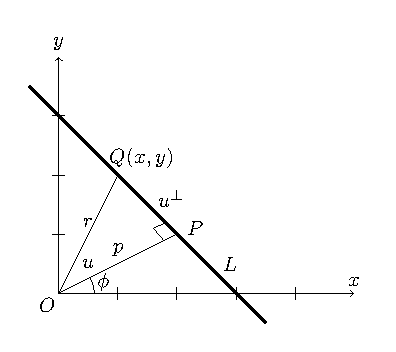
\includegraphics[scale=1]{Imagenes/Figura_Transformada_Radon.eps}
    \caption{Descripción de la línea recta para la definición de la trasformada de Radon.}
    \label{eq:figura_Radon}
\end{figure}
\end{frame}
\begin{frame}
\frametitle{De la Transformada de Radon}
La transformada de Radon de una función $f (x, y)$ de dos variables reales se define por su integral a lo largo de $L$ como:
\begin{align}
\hat{f} (p, \phi) = \mathscr{R} \left\{ f(x, y) \right\} = \scaleint{6ex}_{\bs L} f (x, y) \dd{s}
\label{eq:ecuacion_18_2_1}
\end{align}
\end{frame}
\begin{frame}
\frametitle{Lista de Transformadas Integrales}
\setbeamercolor{item projected}{bg=caribbeangreen,fg=black}
\setbeamertemplate{enumerate items}{%
\usebeamercolor[bg]{item projected}%
\raisebox{1.5pt}{\colorbox{bg}{\color{fg}\footnotesize\insertenumlabel}}%
}
\begin{enumerate}[<+->]
\conti
\item \emph{Transformada Wavelet.}
\\
La transformada Wavelet continua es similar a la transformada de Fourier en el sentido de que se basa en una sola función $\psi$ y que esta función está escalada.
\seti
\end{enumerate}
\end{frame}
\begin{frame}
\frametitle{De la transformada Wavelet}
Pero a diferencia de la transformada de Fourier, también cambiamos la función, generando así una familia de funciones de dos parámetros $\psi_{a, b}$.
\end{frame}
\begin{frame}
\frametitle{De la transformada Wavelet}
Es conveniente definir $\psi_{a, b}$ como sigue:
\pause
\begin{align*}
\psi_{a, b} (x) = \abs{a}^{1/2} \, \psi \left( \dfrac{x - b}{a} \right)
\end{align*}
\end{frame}
\begin{frame}
\frametitle{De la transformada Wavelet}
Entonces la \emph{transformada Wavelet continua} se define por:
\pause
\begin{align*}
(W_{\psi} \, f) (a, b) &= \scaleint{6ex}_{\bs -\infty}^{\infty} f (t) \, \overline{\psi_{a, b} (t)} \dd{t} = \\[0.5em]
&= \abs{a}^{1/2} \, \scaleint{6ex}_{\bs -\infty}^{\infty} f (t) \, \overline{\psi \left( \dfrac{x - b}{a} \right)} \dd{t}
\end{align*}
\end{frame}
\begin{frame}
\frametitle{Sobre la transformada Wavelet}
Traducir al español como tal el término wavelet, nos dejaría alguna de las siguientes opciones:
\setbeamercolor{item projected}{bg=carolinablue,fg=black}
\setbeamertemplate{enumerate items}{%
\usebeamercolor[bg]{item projected}%
\raisebox{1.5pt}{\colorbox{bg}{\color{fg}\footnotesize\insertenumlabel}}%
}
\begin{enumerate}[<+->]
\item Ondícula.
\item Onduleta.
\item Onditas
\end{enumerate}
\end{frame}
\begin{frame}
\frametitle{Sobre la transformada Wavelet}
Siendo claro que en estos casos no es conveniente traducir, ya que al dejar el término en inglés, se mantiene la idea principal, mientras que en español, queda descontextualizado.
\end{frame}
\begin{frame}
\frametitle{Existencia de una Transformada Inversa}
Para cada una de la transformadas integrales listadas, se debe de considerar su correspondiente \textbf{\textcolor{carnelian}{Transformada Inversa}}.
\end{frame}

\section{¿Por qué usar transformadas?}
\frame[allowframebreaks]{\frametitle{Contenido}\tableofcontents[currentsection, hideothersubsections]}
\subsection{Utilidad de las transformadas}

\begin{frame}
\frametitle{Uso de las transformadas}
Como se verá más adelante, aplicar una transformada integral a una EDP es para excluir temporalmente una variable independiente que se ha elegido y dejar de solución de una EDP en una variable menos.
\\
\bigskip
\pause
La solución de esta ecuación será una función de $\alpha$ y las variables restantes.
\end{frame}
\begin{frame}
\frametitle{Cambio de estado y regreso}
Cuando se ha obtenido esta solución, tiene que ser \enquote{invertida} para recuperar la variable \enquote{perdida}.
\end{frame}
\begin{frame}
\frametitle{Cambio de estado y regreso}
Así, si $t$ es la variable eliminada y $g (\alpha)$ es una de las transformaciones dadas anteriormente, \pause obtenemos primero las ecuaciones auxiliares que dan $g$ en términos de $\alpha$ y las variables independientes restantes, resolvemos para $g$ y luego invertimos para obtener $g (\alpha)$.
\end{frame}
\begin{frame}
\frametitle{La transformada inversa}
El proceso de inversión significa, en efecto, la solución de una de las ecuaciones integrales (\ref{eq:ecuacion_7_02}) $\ldots$ (\ref{eq:ecuacion_7_06}), $g (\alpha)$ que se supone conocido y $f (t)$ que se encuentran.
\end{frame}
\begin{frame}
\frametitle{Descripción gráfica de las transformadas}
\usetikzlibrary{shapes.multipart}
\begin{figure}
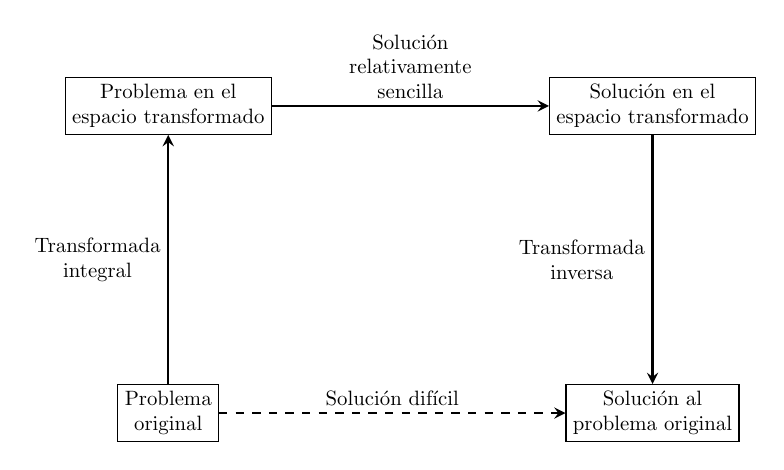
\begin{tikzpicture}[every text node part/.style={align=center}, >=stealth, node distance = 8.2cm, auto, every node/.style={scale=0.75}]
	\node (cuadro1) [rectangle, draw] {Problema \\ original}; \pause
	\node (cuadro2) [right of = cuadro1, rectangle, draw] {Solución al \\ problema original}; \pause
    \path [->, dashed, thick] (cuadro1) edge node [above, midway] {Solución difícil} (cuadro2); \pause
    
    \node (cuadro3) [above of = cuadro1, yshift=-3cm, rectangle, draw] {Problema en el \\ espacio transformado}; \pause
	\path [->, thick] (cuadro1) edge node[left, midway] {Transformada \\ integral} (cuadro3); \pause
    
    \node (cuadro4) [right of = cuadro3, rectangle, draw] {Solución en el \\ espacio transformado}; \pause
    \path [->, thick] (cuadro3) edge node [above=-0.3, midway] {Solución \\ relativamente \\ sencilla} (cuadro4); \pause

	\path [->, thick] (cuadro4) edge node[left, midway] {Transformada \\ inversa}  (cuadro2);
	
\end{tikzpicture}
\end{figure}
\end{frame}
\begin{frame}
\frametitle{Soluciones con las transformadas}
Tales soluciones son conocidas y pueden ser obtenidos formalmente del teorema de la integral de Fourier.
\end{frame}

\section{Propiedades de las Transformadas}
\frame[allowframebreaks]{\frametitle{Contenido}\tableofcontents[currentsection, hideothersubsections]}
\subsection{Linealidad de las TI}

\begin{frame}
\frametitle{Linealidad de las transformadas}
Todas estas transformadas integrales son lineales, por lo que satisfacen las siguientes propiedades:
\pause
\begin{eqnarray}
\begin{aligned}[b]
&\scaleint{6ex}_{\bs a}^{b} [ c_{1} \, f_{1} (t) + c_{2} \, f_{2} (t)] \; K(\alpha, t) \, \dd{t} = \\[0.5em] \pause
&= c_{1} \, \scaleint{6ex}_{\bs a}^{b} f_{1} (t) \; K (\alpha, t) \, \dd{t} + \\
&+ c_{2} \, \scaleint{6ex}_{\bs a}^{b} f_{2} (t) \; K (\alpha, t) \, \dd{t}
\end{aligned}
\label{eq:ecuacion_15_08} 
\end{eqnarray}
\end{frame}
\begin{frame}
\frametitle{Linealidad de las tranformadas}
% Además de:
% \pause
% \begin{align}
% \scaleint{6ex}_{\bs a}^{b}  c \; f (t) \; K (\alpha, t) \, \dd t =  c \; \scaleint{6ex}_{\bs a}^{b} f (t) \; K (\alpha, t) \, \dd{t}
% \label{eq:ecuacion_15_09}
% \end{align}
% \pause
Donde $c_{1}$ y $c_{2}$ son constantes y $f_{1} (t)$ y $f_{2} (t)$ son funciones para las cuales la operación transformada está definida.
\end{frame}
\begin{frame}
\frametitle{Las transformadas como operador}
Representando la transformada integral lineal por el operador $\mathcal{L}$, obtenemos:
\pause
\begin{align}
g (\alpha) = \mathcal{L} \, f (t)
\label{eq:ecuacion_15_10}
\end{align}
\end{frame}
\begin{frame}
\frametitle{Operador inverso}
Uno espera que exista el operador inverso $\mathcal{L}^{-1}$, de manera tal que:
\pause
\begin{align}
f (t) = \mathcal{L}^{-1}  \; g (\alpha)
\label{eq:ecuacion_15_11}
\end{align}
\end{frame}
\begin{frame}
\frametitle{Complicaciones obteniendo el operador inverso}
En general, el mayor problema con el uso de las transformadas integrales, es determinar el operador inverso.
\\
\bigskip
\pause
Sin embargo, para los dos tipos de transformaciones: de Fourier y de Laplace, obtener la transformada inversa es relativamente sencillo.
\end{frame}

% %Ref. Patra (2018) 1.2 Classes of functions.
\section{Tipos de funciones}
\frame[allowframebreaks]{\frametitle{Contenido}\tableofcontents[currentsection, hideothersubsections]}
\subsection{Base matemática}

\begin{frame}
\frametitle{Funciones y clases}
Una función de valor único $f (x)$ de la variable independiente $x$ que es continua en un intervalo $[a, b]$, se dice que pertenece a una clase denotada por $f \in C \, [a, b]$.
\end{frame}
\begin{frame}
\frametitle{Función continua}
Se dice que una función $f (x)$ es continua por partes en un intervalo $(a, b)$, \pause si el intervalo se puede dividir en un número finito de subintervalos que no se intersectan $(a, a_{1}), (a_{1}, a_{2}), \ldots, (a_{n -1}, b)$.
\end{frame}
\begin{frame}
\frametitle{Función continua}
En cada uno de los subintervalos
\begin{align*}
(a, a_{1}), (a_{1}, a_{2}), \ldots, (a_{n -1}, b)
\end{align*}
la función es continua y tiene límites finitos cuando $x$ se acerca a los puntos extremos de cada uno de los subintervalos.
\end{frame}
\begin{frame}
\frametitle{Función continua de clase $P$}
Se dice que dicha función pertenece a una clase denotada por $f \in P \, (a, b)$.
\\
\bigskip
\pause
Una función continua a trozos $f$ en $(a, b)$, cuya derivada de primer orden es también una función continua a trozos en $(a, b)$ y pertenece a una clase denotada por $f \in P^{1} \, (a, b)$.
\end{frame}
\begin{frame}
\frametitle{Funciones integrables}
Se dice que el conjunto de funciones $f (x)$ es absolutamente integrable sobre $\Omega$, si:
\pause
\begin{align*}
\scaleint{6ex}_{\bs \Omega}  \abs{f (x)} \dd{x}
\end{align*}
es finito.
\end{frame}
\begin{frame}
\frametitle{Funciones con integrales finitas}
Entonces decimos que esta función pertenece a una clase denotada por $f (x) \in A_{1} (\Omega)$.
\\
\bigskip
\pause
De manera similar, el hecho que $f \in A_{m} (\Omega)$ implica que:
\begin{align*}
\scaleint{6ex}_{\bs \Omega}  \abs{f (x)} \dd{x}
\end{align*}
es finito.
\end{frame}
\begin{frame}
\frametitle{Funciones particulares}
Finalmente, presentamos una clase de funciones $f (x)$, que satisface las siguientes condiciones:
\pause
\setbeamercolor{item projected}{bg=ceil,fg=black}
\setbeamertemplate{enumerate items}{%
\usebeamercolor[bg]{item projected}%
\raisebox{1.5pt}{\colorbox{bg}{\color{fg}\footnotesize\insertenumlabel}}%
}
\begin{enumerate}[<+->]
\item $f (x)$ se define en $c < x < c + 2 \, l$.
\item $f (x)$ es una función periódica del período $2 \, l$.
\seti
\end{enumerate}
\end{frame}
\begin{frame}
\frametitle{Funciones particulares}
\setbeamercolor{item projected}{bg=ceil,fg=black}
\setbeamertemplate{enumerate items}{%
\usebeamercolor[bg]{item projected}%
\raisebox{1.5pt}{\colorbox{bg}{\color{fg}\footnotesize\insertenumlabel}}%
}
\begin{enumerate}[<+->]
\conti
\item $f (x)$ y $\pderivada{f} (x)$ son continuas por partes en $c  < x <c + 2 \, l$ expresado por $f (x) \in P^{1} (c, c + 2 \, l)$.
\end{enumerate}
\pause
Se dice que esta clase de función $f (x)$ satisface las condiciones de Dirichlet. 
\end{frame}
\begin{frame}
\frametitle{Funciones de orden exponencial}
Se dice que una función $f (x)$ es de orden exponencial $\sigma$ cuando $x \to \infty$, si las constantes $\sigma, m (> 0)$ se pueden encontrar de modo que:
\pause
\begin{eqnarray*}
\begin{aligned}
\abs{ e^{\sigma \, x} \, f (x)} < m \pause \hspace{0.3cm} \Longrightarrow \hspace{0.3cm} \abs{f (x)} < m \, e^{m \, \sigma} \pause \hspace{0.3cm} x > x_{0}
\end{aligned}
\end{eqnarray*}
%De manera equivalente, también se puede escribir $f (x) = 0 \, (e^{m \, \sigma})$ mientras $x \to \infty$.
\end{frame}


% %Ref. Patra (2018) 1.3 Series de Fourier y la Fórmula Integral de Fourier.

\section{Fórmula integral de Fourier}
\frame[allowframebreaks]{\frametitle{Contenido}\tableofcontents[currentsection, hideothersubsections]}
\subsection{Series de Fourier}

\begin{frame}
\frametitle{Función y series de Fourier}
Consideremos una función $f (x)$ que satisface las condiciones de Dirichlet en el intervalo $[-l, l]$, \pause la función pertenece a la clase $P^{1} (R)$ \pause y también a la clase $A_{1} (R)$.
\end{frame}
\begin{frame}
\frametitle{Función y series de Fourier}
Sea el período principal de $f (x)$ igual a $2 \, l$. 
\\
\bigskip
\pause
Entonces $f (x)$ admite una representación en una serie de Fourier:
\pause
\begin{align*}
f (x) = a_{0} + \nsum_{n=1}^{\infty} \left[ a_{n} \, \cos \left( \dfrac{n \pi x}{l}  \right) + b_{n} \, \sin \left( \dfrac{n \pi x}{l}  \right) \right]
\end{align*}
\end{frame}
\begin{frame}
\frametitle{Coeficientes de la serie de Fourier}
Donde los coeficientes son:
\pause 
\begin{align*}
a_{0} &= \dfrac{1}{2 \, l} \scaleint{6ex}_{\bs -l}^{l} f (x) \dd{x} \\[0.5em]
(a_{n}, b_{n}) &= \dfrac{1}{l} \scaleint{6ex}_{\bs -l}^{l} f (x) \left[ \cos \left( \dfrac{n \, \pi \, x}{l} \right), \sin \left( \dfrac{n \, \pi \, x}{l} \right) \right] \dd{x}
\end{align*}
\end{frame}
\begin{frame}
\frametitle{Tomando la diferencia entre coeficientes}
Entonces cuando:
\pause
\begin{eqnarray*}
\begin{aligned}
a_{n} - i \, b_{n} = \pause \dfrac{1}{l} \scaleint{6ex}_{\bs -l}^{l} f (x) \, \exp \left( - \dfrac{i \, n \, \pi \, x}{l} \right) \dd{x}
\end{aligned}
\end{eqnarray*}
\end{frame}
\begin{frame}
\frametitle{Nuevos coeficientes}
Definimos a continuación:
\pause
\begin{eqnarray*}
\begin{aligned}
a_{0} &= c_{0} \\[0.5em] \pause
a_{n} &= c_{n} + c_{-n} \\[0.5em] \pause
i \, b_{n} &= c_{n} - c_{-n}
\end{aligned}
\end{eqnarray*}
\end{frame}
\begin{frame}
\frametitle{Represetación de la función}
Entonces tendremos que:
\pause
\begin{eqnarray}
\begin{aligned}[b]
f (x) &= c_{0} {+} \nsum_{n=1}^{\infty} \bigg[ c_{n} \, \exp \left( -\dfrac{i n \pi x}{l} \right) + \\[0.5em]
&+ c_{-n} \, \exp \left( \dfrac{i n \pi x}{l} \right) \bigg] = \\[0.5em] \pause
&= \nsum_{-\infty}^{+\infty} c_{n} \, \exp \left( - \dfrac{i \, n \, \pi \, x}{l} \right)
\end{aligned}
\label{eq:ecuacion_01_02}
\end{eqnarray}
\end{frame}
\begin{frame}
\frametitle{Coeficientes de la representación}
Donde el coeficiente $c_{n}$ es:
\pause
\begin{eqnarray}
\begin{aligned}[b]
c_{n} &= \dfrac{1}{2 \, l} \scaleint{6ex}_{\bs -l}^{l} f (x) \, \exp \left( \dfrac{i \, n \, \pi \, x}{l} \right) \dd{x} = \\[0.5em] \pause
&= \dfrac{1}{2 \, l} \scaleint{6ex}_{\bs -l}^{l} f (t) \, \exp \left( \dfrac{i \, n \, \pi \, t}{l} \right) \dd{t}
\end{aligned}
\label{eq:ecuacion_01_03}
\end{eqnarray}
\pause
Esta es forma de la serie de Fourier se le llama \textocolor{byzantine}{forma compleja de la serie de Fourier} en el intervalo $(-l , l)$.
\end{frame}
\begin{frame}
\frametitle{La función y la suma de integrales}
Por lo que de las ecs. (\ref{eq:ecuacion_01_02}) y (\ref{eq:ecuacion_01_03}), se obtiene:
\pause
\begin{eqnarray}
\begin{aligned}[b]
f (x) &= \nsum_{-\infty}^{+\infty} \left[ \dfrac{1}{2 \, l} \scaleint{6ex}_{\bs -l}^{l} f (t) \exp \left( \dfrac{i \, n \, \pi \, t}{l} \right) \dd{t} \right] \times \\[0.5em]
&\times \exp \left( - \dfrac{i \, n \, \pi \, x}{l} \right)
\label{eq:ecuacion_01_04}
\end{aligned}
\end{eqnarray}
\end{frame}
\begin{frame}
\frametitle{Haciendo cambio de variable}
Ahora hagamos el siguiente cambio de variable:
\pause
\begin{align*}
\dfrac{\pi}{l} = \delta \xi
\end{align*}
\pause
Notemos que $\delta \xi \to 0$ mientras $l \to \infty$, tal que $l \, \delta \xi = \pi =$ un número finito.
\end{frame}
\begin{frame}
\frametitle{La función con el cambio de variable}
Entonces la serie (\ref{eq:ecuacion_01_04}), antes de tomar el límite cuando $\delta \xi \to 0$, se convierte en:
\pause
\begin{align*}
f (x) &= \dfrac{1}{2 \, \pi} \nsum_{-\infty}^{+\infty} \delta \xi \, \left[ \scaleint{6ex}_{\bs -\frac{\pi}{\delta \xi}}^{\frac{\pi}{\delta \xi}} f (t) \, \exp \left( i \, n \, t \, \delta \xi \right) \dd{t} \right] \times \\[0.5em]
&\times \exp \left( - i \, n \, x \, \delta \xi \right) = 
\end{align*}
\end{frame}
\begin{frame}
\frametitle{La función con el cambio de variable}
\begin{align*}
f (x) = \dfrac{1}{2 \, \pi} \scaleint{6ex}_{\bs -\frac{\pi}{\delta \xi}}^{\frac{\pi}{\delta \xi}} f (t) \, \left[ \nsum_{-\infty}^{+\infty} \delta \xi \, \exp \left( i \, n (t - x \, \delta \xi) \right) \right] \dd{t}
\end{align*}
después de intercambiar formalmente los signos de suma e integración.
\end{frame}
\begin{frame}
\frametitle{La clase de la función}
Dado que asumimos que  $f (x) \in P^{1} (R)$ \pause y también que $f (x) \in A_{1} (R)$, \pause haciendo que $\delta \xi \to 0$ y usando la definición de integral definida de Riemann como límite de una suma obtenemos:
\end{frame}
\begin{frame}
\frametitle{La clase de la función}
\begin{eqnarray}
\begin{aligned}
f (x) &= \dfrac{1}{2 \, \pi} \scaleint{6ex}_{\bs -\infty}^{\infty} f (t) \, \left[ \exp \left( i (t - x) \, y \right) \, \dd{y} \right] \dd{t} \label{eq:ecuacion_01_05} \\[0.5em] \pause 
\Rightarrow f (x) &= \dfrac{1}{\sqrt{2 \, \pi}} \scaleint{6ex}_{\bs -\infty}^{\infty} \exp \left( i \, y \, x \right) \big[ F (y) \big] \dd{y} \label{eq:ecuacion_01_06} \\[0.5em] \pause
\mbox{donde} \hspace{0.5cm} F (y) &= \dfrac{1}{\sqrt{2 \, \pi}} \scaleint{6ex}_{\bs -\infty}^{\infty} f (t) \, \exp \left( i \, y \, t \right) \dd{t} \label{eq:ecuacion_01_07}
\end{aligned}
\end{eqnarray}
\end{frame}
\begin{frame}
\frametitle{Ocupando el coseno}
De nueva cuenta, de la ec. (\ref{eq:ecuacion_01_05}), se obtiene lo siguiente:
\pause
\begin{align}
f (x) = \dfrac{1}{\pi} \scaleint{6ex}_{\bs 0}^{\infty}  \dd{y} \, \scaleint{6ex}_{\bs -\infty}^{+\infty} f (t) \, \cos y (-t + x) \dd{t} \label{eq:ecuacion_01_08}
\end{align}
\pause
La ecuación (\ref{eq:ecuacion_01_08}) se le conoce como la \textocolor{cadetblue}{fórmula integral de Fourier}.
\end{frame}
\begin{frame}
\frametitle{Cuando hay discontinuidades}
En un punto de discontinuidad finita de $f (x)$, el lado izquierdo de la ec. (\ref{eq:ecuacion_01_08}) se reemplaza con:
\pause
\begin{align*}
\dfrac{1}{2} \big[ f (x + 0) + f (x - 0) \big]
\end{align*}
en el sentido de los valores límite.
\end{frame}
\end{document}